\section{Resultate
	\label{ableitung:section:resultate}}
\rhead{Resultate}
Die Resultate dieser Arbeit sollen hauptsächlich aufzeigen, ob das vorgestellte Verfahren der finiten Differenzen für die Optimierung eines neuronalen Netzwerks geeignet ist. Um dies experimentel zu belegen wurde einfaches Netzwerk gewählt um die logische XOR Verknüpfung zu trainieren.
\begin{figure}[h]
	 \centering
\begin{tabular}{cc}
	\begin{tikzpicture}
	
	\node (x1) at (0, 0.75) {$x_1$};
	\node (x2) at (0, 1.25) {$x_2$};
	\node (y) at (3, 1) {$y$};
	
	\node[xor gate US, draw] at ($(x1) + (1.5, 0.25)$) (notx) {};
	
	\draw (x1) -- (notx);
	\draw (x2) -- (notx);

	\draw (notx.output) -- (y);
	
	
	\end{tikzpicture}	
	&
	\begin{tabular}{cc|c}
		\hline
		$x_1$ & $x_2$ & $y$ \\
		\hline
		0 & 0 & 0 \\ 
		0 & 1 & 1 \\ 
		1 & 0 & 1 \\ 
		1 & 1 & 0 \\
		\hline						
	\end{tabular}
\end{tabular}
\end{figure}



\tikzstyle{inputNode}=[draw,circle,minimum size=17pt,inner sep=0pt]
\tikzstyle{stateTransition}=[-stealth, thick]
\begin{figure}
	\centering
	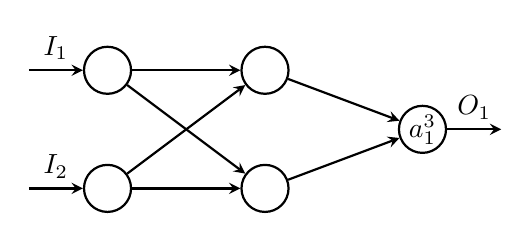
\begin{tikzpicture}
	
	\node[inputNode, thick] (i1) at (5, 1.5) {};
	\node[inputNode, thick] (i2) at (5, 0) {};
	
	\node[inputNode, thick] (h1) at (7, 1.5) {};
	\node[inputNode, thick] (h2) at (7, 0) {};
	
	\node[inputNode, thick] (o1) at (9, 0.75) {$a^{3}_{1}$};
	
	\draw[stateTransition] (4, 1.5) -- node[above] {$I_1$} (i1);
	\draw[stateTransition] (4, 0) -- node[above] {$I_2$} (i2);
	
	
	\draw[stateTransition] (i1) -- (h1);
	\draw[stateTransition] (i1) -- (h2);
	\draw[stateTransition] (i2) -- (h1);
	\draw[stateTransition] (i2) -- (h2);
	
	\draw[stateTransition] (h1) -- (o1);
	\draw[stateTransition] (h2) -- (o1);
	
	\draw[stateTransition] (o1) -- node[above] {$O_1$} (10, 0.75);
	\end{tikzpicture}
\end{figure}

Das Netzwerk wurde mittels Gradientenabstiegverfahren in Facebook PyTorch trainiert. Weiter wurde in PyTorch die Methode der finiten Differenzen implementiert und das Netzwerk mit einer unterschiedlichen Anzahl Stützstellen und eine unterschiedlichen Abstand der Stützstellen $h$ trainiert.
Die Resultate sind in den Abbildungen \ref{ableitung:fig:xor_h1}, \ref{ableitung:fig:xor_h01}, \ref{ableitung:fig:xor_h1} ersichtlich, die y-Achse stellt den quadratischen Fehler zwischen $\hat{y}$ und $y$ dar, während die x-Achse die Entwicklung über die Anzahl Epochen aufzeigt.

\begin{figure}
	\begin{tikzpicture}
	\begin{semilogyaxis}[xmin=0, xmax=1000, ymin=10e-15, ymax=10, width=\textwidth, height=0.30\textheight]
	\addplot[one, line width=1pt] table [x=epoch, mark=none, y=loss, col sep=comma] {papers/ableitung/data/backprop.csv};
	\addplot[two] table [x=epoch, mark=none, y=loss, col sep=comma] {papers/ableitung/data/h1-support2.csv};
	\addplot[three] table [x=epoch, mark=none, y=loss, col sep=comma] {papers/ableitung/data/h1-support4.csv};
	\addplot[four] table [x=epoch, mark=none, y=loss, col sep=comma] {papers/ableitung/data/h1-support6.csv};
	\addplot[five] table [x=epoch, mark=none, y=loss, col sep=comma] {papers/ableitung/data/h1-support8.csv};
	
	\addlegendentry{Backprop}	
	\addlegendentry{Support: 2}
	\addlegendentry{Support: 4}
	\addlegendentry{Support: 6}
	\addlegendentry{Support: 8}
	
	
	\end{semilogyaxis}
	\end{tikzpicture}
	\caption{Resultate des Gradientenabstiegs mit Stützstellenabstand $h=1$.}
	\label{ableitung:fig:xor_h1}
\end{figure}

\begin{figure}	
	\begin{tikzpicture}
	\begin{semilogyaxis}[xmin=0, xmax=1000, ymin=10e-15, ymax=10, width=\textwidth, height=0.3\textheight]
	\addplot[one, line width=1pt] table [x=epoch, mark=none, y=loss, col sep=comma] {papers/ableitung/data/backprop.csv};
	\addplot[two] table [x=epoch, mark=none, y=loss, col sep=comma] {papers/ableitung/data/h01-support2.csv};
	\addplot[three] table [x=epoch, mark=none, y=loss, col sep=comma] {papers/ableitung/data/h01-support4.csv};
	\addplot[four] table [x=epoch, mark=none, y=loss, col sep=comma] {papers/ableitung/data/h01-support6.csv};
	\addplot[five] table [x=epoch, mark=none, y=loss, col sep=comma] {papers/ableitung/data/h01-support8.csv};
	
	\addlegendentry{Backprop}	
	\addlegendentry{Support: 2}
	\addlegendentry{Support: 4}
	\addlegendentry{Support: 6}
	\addlegendentry{Support: 8}
	
	
	\end{semilogyaxis}
	\end{tikzpicture}
	\caption{Resultate des Gradientenabstiegs mit Stützstellenabstand $h=0.1$.}
	\label{ableitung:fig:xor_h01}
\end{figure}
	
\begin{figure}
	\begin{tikzpicture}
	\begin{semilogyaxis}[xmin=0, xmax=1000, ymin=10e-15, ymax=10, width=\textwidth, height=0.3\textheight]
	\addplot[one, line width=1pt] table [x=epoch, mark=none, y=loss, col sep=comma] {papers/ableitung/data/backprop.csv};
	\addplot[two] table [x=epoch, mark=none, y=loss, col sep=comma] {papers/ableitung/data/h001-support2.csv};
	\addplot[three] table [x=epoch, mark=none, y=loss, col sep=comma] {papers/ableitung/data/h001-support4.csv};
	\addplot[four] table [x=epoch, mark=none, y=loss, col sep=comma] {papers/ableitung/data/h001-support6.csv};
	\addplot[five] table [x=epoch, mark=none, y=loss, col sep=comma] {papers/ableitung/data/h001-support8.csv};
	
	\addlegendentry{Backprop}	
	\addlegendentry{Support: 2}
	\addlegendentry{Support: 4}
	\addlegendentry{Support: 6}
	\addlegendentry{Support: 8}
	
	
	\end{semilogyaxis}
	\end{tikzpicture}
	\caption{Resultate des Gradientenabstiegs mit Stützstellenabstand $h=0.01$.}
		\label{ableitung:fig:xor_h001}
\end{figure}
	